\chapter{Slovník pojmů}
\label{priloha-A}

\renewcommand*{\arraystretch}{1.4}
\begin{longtable}{p{3cm}p{11.2cm}}
Backend & Část aplikace obsahující její logiku. Typicky běží na~serveru a uživatel do~ní nevidí.\\

Klient & Aplikace běžící na~straně uživatele.\\

Kontrolér & V~kontextu webového api přijímá požadavky na~službu a vrací odpovědi. Akce kontroléru k~vykonání je specifikována v~url požadavku.\\

Kubernetes & Open-source platforma pro~správu a nasazení kontejnerizovaných aplikací.\\

Dataframe & Dvou-dimenzionální datová struktura tabulkového stylu s~pojmenovanými sloupci.\\

Dataset & Kolekce dat, nad~kterými se vykonává analýza.\\

Framework & Software, který obsahuje a poskytuje pomocné prvky k~vývoji nových aplikací.\\

Log & Záznam o~činnost.\\

Logger & Objekt implementující ILogger rozhraní schopný vytvářet logy.\\

NuGet & Instalační balíček knihovny či rozšíření pro~.NET projekty.\\

Open-source & Software, který bývá typicky zdarma a jehož zdrojové kódy jsou veřejně dostupné.\\

Outlier & Hodnota výrazně se lišící od~ostatních v~dané kolekci dat.\\

RabitMQ & Open-source software zprostředkovávající zprávy mezi částmi distribuovaných systémů.\\

Routing & V~kontextu webového API se jedná o~směrování požadavků. Mapuje požadavky na~konkrétní kontroléry a jejich akce.\\

Výjimka & V~kontextu programování se jedná o~výjimečnou situaci, typicky chybu. \\

Widget & Ovladatelný prvek grafického uživatelského rozhraní.\\

XPlot & Vizualizační knihovna pro~jazyk F\#, který lze díky kompatibilitě .NET platformy omezeně použít i v~C\#.
\end{longtable}

\chapter{Seznam zkratek}
\label{priloha-B}

\renewcommand*{\arraystretch}{1.4}
\begin{longtable}{p{2cm}p{12.2cm}}
API & Application Programming Interface (Rozhraní pro~programování aplikací)\newline
Rozhraní, jež umožňuje používat funkce nebo části softwarového systému.\\

CSV & Comma Separated Values (Hodnoty oddělené čárkou)\newline
Typ datového souboru, ve~kterém je na~každém řádku jeden záznam, jehož hodnoty jsou odděleny čárkou.\\

DBSCAN & Density based spatial clustering of applications with noise\newline
Shlukovací algoritmus strojového učení.\\

DI & Dependency Injection (Vkládání závislostí)\newline
Návrhový vzor pro~získávání objektů jinému objektu, na~kterých tento závisí.\\

GELF & Graylog Extended Log Format (Rozšířený formát logů Graylogu)\newline
Logovací poskytovatel pro~Graylog.\\

GMM & Gaussian Mixture Model (Směs Gaussových rozložení)\newline
Shlukovací a klasifikační algoritmus strojového učení.\\

HDBSCAN & Hierarchical density based spatial clustering of applications with noise\newline
Shlukovací algoritmus strojového učení.\\

JSON & JavaScript Object Notation (Objektová notace jazyka JavaScript)\newline
Formát pro serializaci a přenos dat.\\

MinPts & Minimum points (Minimální počet bodů)\newline
Parametr algoritmu DBSCAN určující minimální počet bodů, od~kterého se prostor považuje za~hustý.\\

MRD & Mutual Reachability Distance (Vzdálenost vzájemné dosažitelnosti)\newline
Typ vzdálenosti používající se algoritmem HDBSCAN.\\

OPTICS & Ordering Points to Identify Cluster Structure\newline
Shlukovací algoritmus strojového učení.\\

RD & Reachability Distance (Vzdálenost dosažitelnosti)\newline
Typ vzdálenosti používající se algoritmem OPTICS.\\

REST & Representational State Transfer (Přenost reprezentativního stavu)\newline
Typ architektury využívaný pro webové služby.\\

ROI & Return of Investment (Návratnost investice)\newline
Poměr zisku a investice.\\

RPA & Robotic Process Automation (Robotická automatizace procesů)\newline
Jedná se o~provádění akcí tzv. boty nebo-li softwarovými roboty za~účelem automatizace.\\

RQA & Robotic Quality Assurance (Robotické zajištění jakosti)\newline
Systém firmy Y~Soft pro~robotické automatizované testování.\\

SOM & Self-Organizing Maps\newline
Shlukovací algoritmus strojového učení.\\
   
QA & Quality Assurance (Zajištění jakosti)\newline
Obor zabývající se plánováním a vylepšováním procesů.\\

UI & User Interface (Uživatelské rozhraní)\newline
Část aplikace určená pro~interakci člověka s~počítačem.\\
   
\end{longtable}

\chapter{Vývojový diagram dávkového stahování logů z~Graylogu}
\label{priloha-C}

\begin{figure}[tbh]
	\centering
	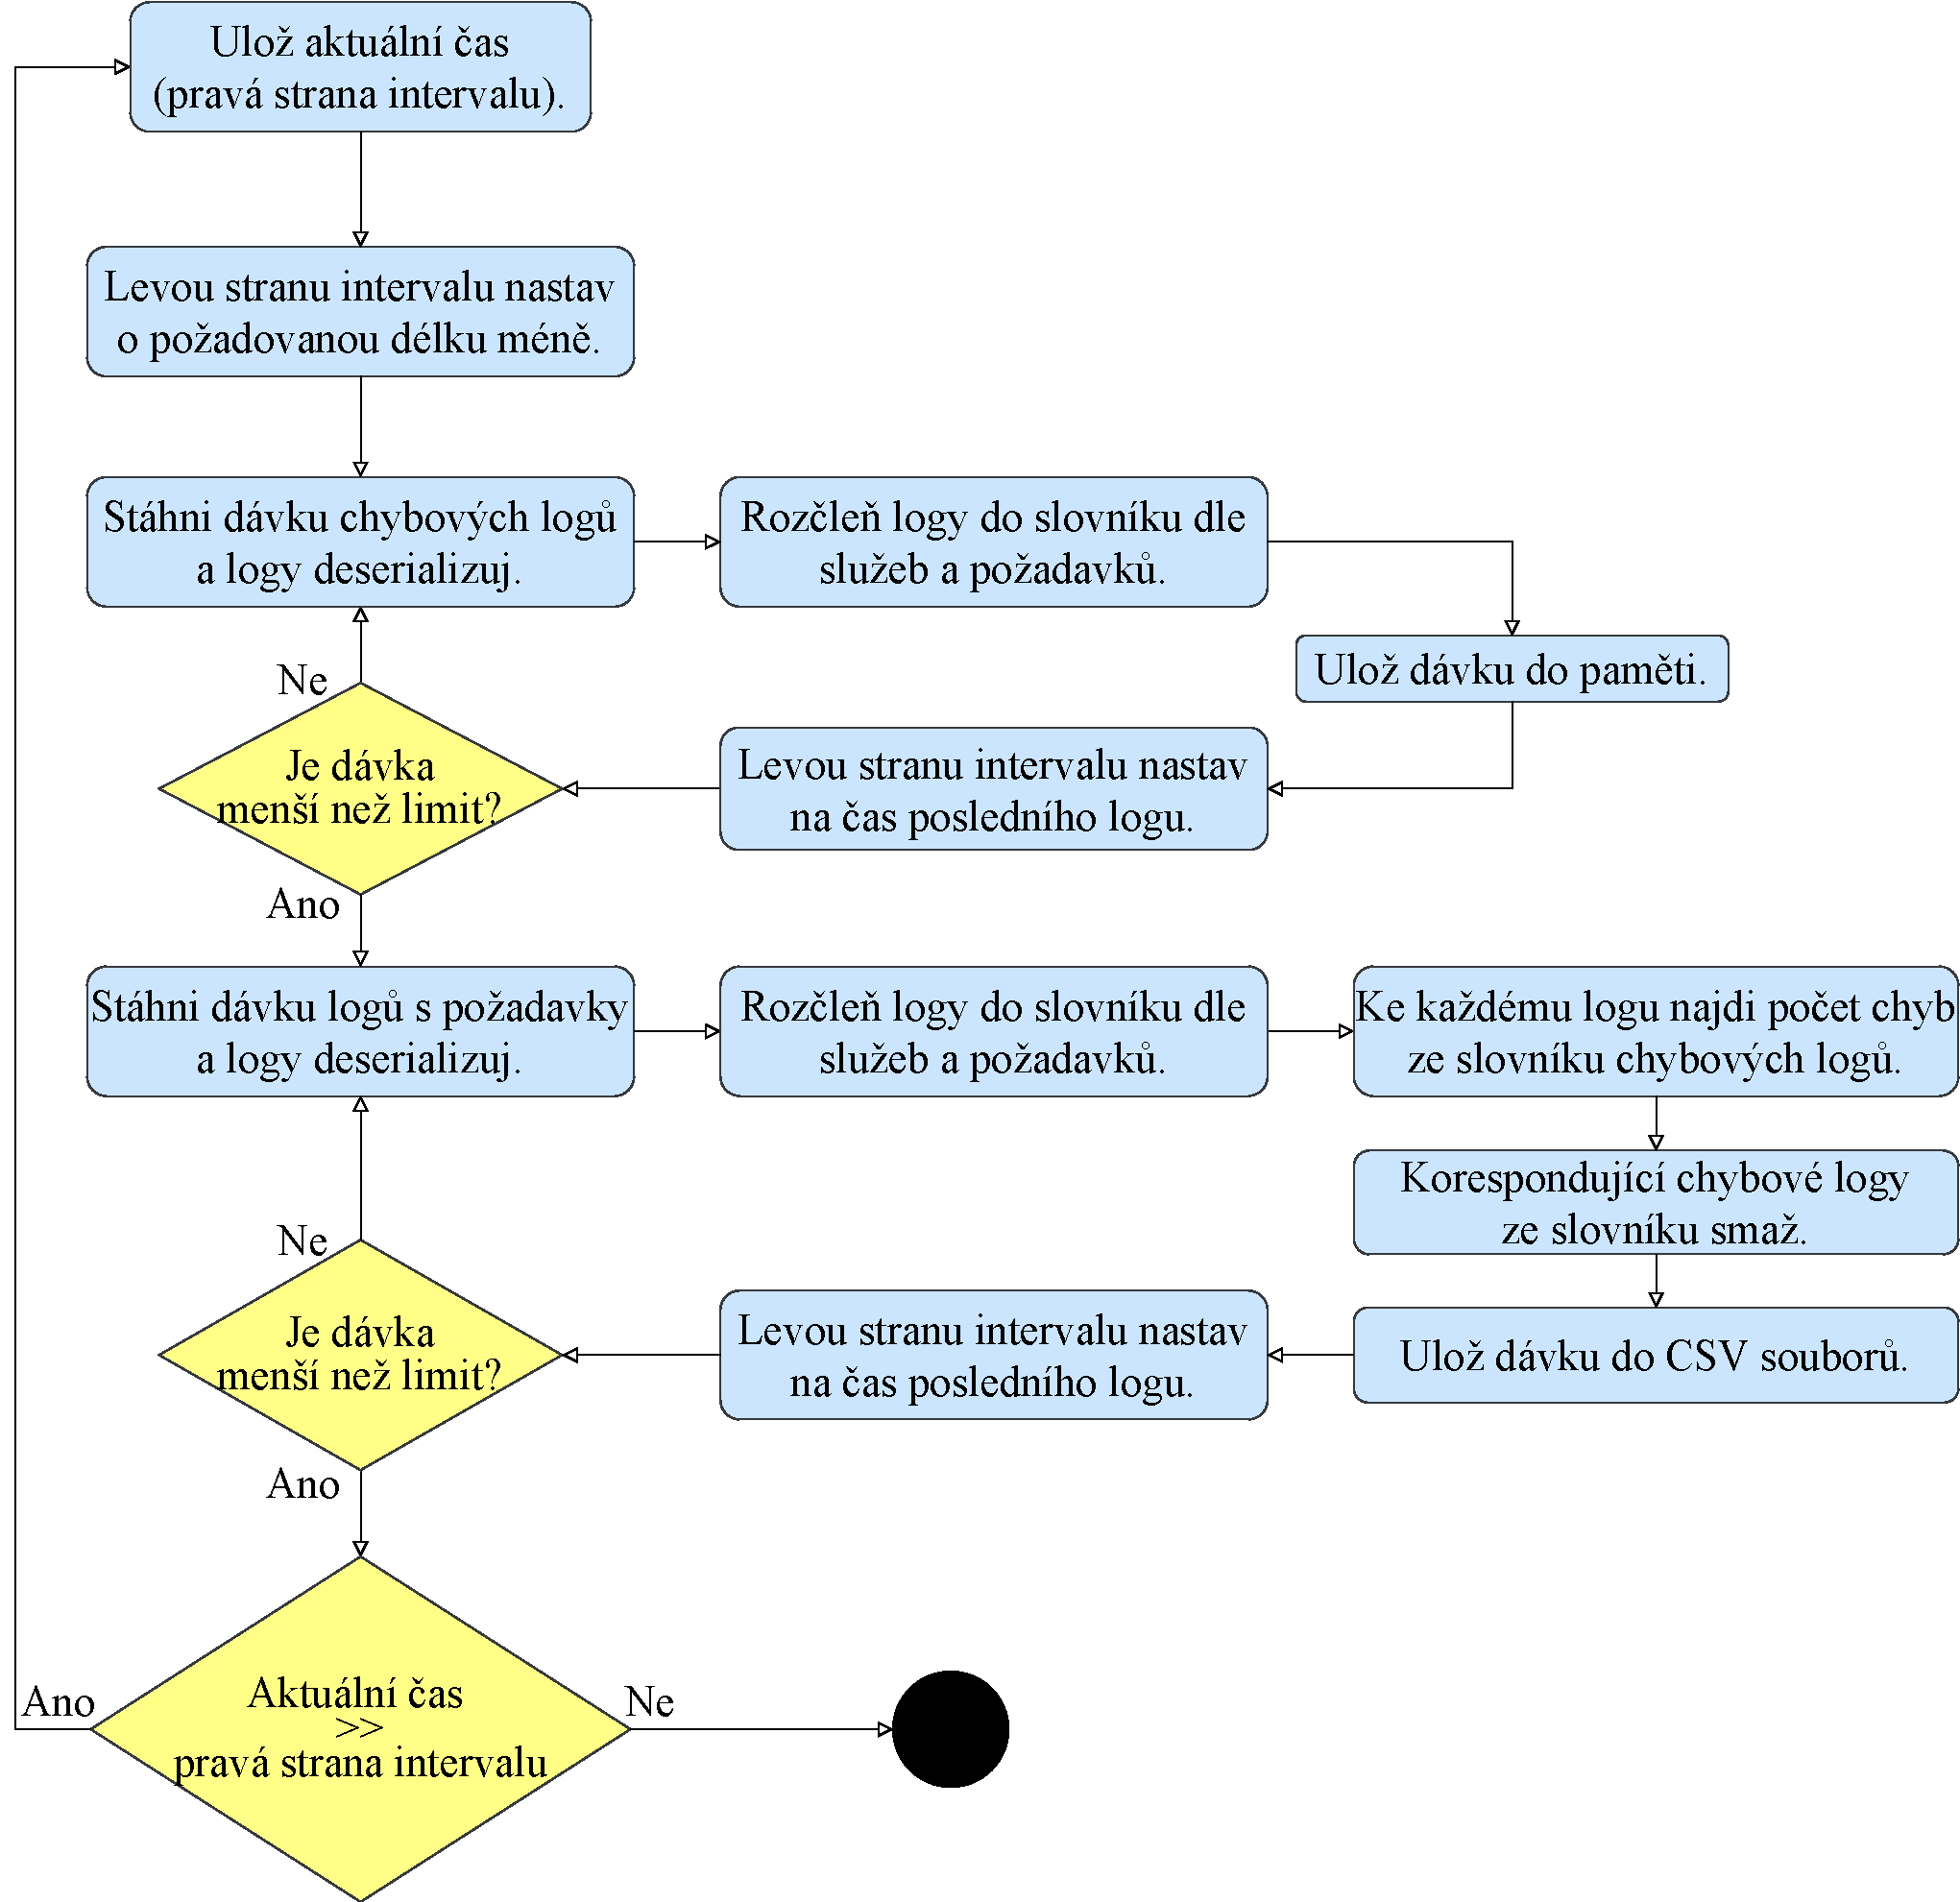
\includegraphics[width=0.97\textwidth]{obrazky/graylog-download-algorithm.pdf}
	\caption{Algoritmus dávkového stahování logů z~Graylogu}
\end{figure}

\chapter{Posudek firmy Y~Soft na~řešení detekce anomálií}
\label{priloha-D}
\begin{figure}[tbh]
	\centering
	
\includegraphics[width=1\textwidth]{obrazky/posudek-ysoft.pdf}
	\caption{Posudek firmy Y~Soft na~řešení detekce anomálií}
\end{figure}

\chapter{Obsah přiloženého paměťového média}
\label{priloha-E}

\begin{itemize}
  \item \texttt{/build} --- Přeložené řešení
  \item \texttt{/demo} --- Jupyter notebooky s~demonstrací řešení
    \begin{itemize}
        \item \texttt{/csv\_examples} --- Ukázkové CSV soubory s~vygenerovanými daty
    \end{itemize}
  \item \texttt{/doc} --- Dokumentace k~řešení
    \begin{itemize}
        \item \texttt{/latex} --- Zdrojové soubory technické zprávy
        \item \texttt{technicka\_zprava.pdf} --- Text bakalářské práce
    \end{itemize}
  \item \texttt{/nuget} --- NuGet balíčky knihoven řešení
  \item \texttt{/src} --- Zdrojové kódy řešení
  \item \texttt{README.md} --- Popis obsahu média a návod k použití
\end{itemize}